\subsection{Bootstrap}

\indent 

The bootstrap is a flexible and powerful statistical tool that can be used to quantify the uncertainty associated with a given estimator or statistical learning method.

\subsubsection{Simple example}

\indent 

Suppose that we wish to invest a fixed sum of money in two financial assets that yield returns of $X$ and $Y$ where $X$ and $Y$ are random quantities.

The goal is to create a portfolio by investing fraction $\alpha$ of our wealth in $X$ and $(1-\alpha)$ in $Y$.

Want to choose to minimise the total risk of the investment. Mathematically, this involves minimising the variance of our investment portfolio $\text{Var}(\alpha X+(1-\alpha)Y)$.

The solution to this problem (via calculus) is:

\begin{align*}
    \alpha = \frac{\sigma_Y^2 -\sigma_{XY}}{\sigma_X^2+\sigma_Y^2 - 2\sigma_{XY}}
\end{align*}

where $\sigma_X^2 = \text{Var}(X)$, $\sigma_Y^2 = \text{Var}(Y)$, $\sigma_{XY}^2 = \text{Cov}(X,Y)$.

\subsubsection{Experiment}

\indent

The values of $\sigma_X^2,\sigma_Y^2$, and $\sigma_{XY}$ are unknown but estimates can be computed from the data.

The estimate of $\alpha$ that minimises the variance of the investment can then be computed with

\begin{align*}
    \widehat{\alpha} = \frac{\widehat{\sigma}_Y^2 -\widehat{\sigma}_{XY}}{\widehat{\sigma}_X^2+\widehat{\sigma}_Y^2 - 2\widehat{\sigma}_{XY}}
\end{align*}

Suppose that $X$ and $Y$ can be sampled from the population repeatedly. 

You sample 100 pairs of $(X,Y)$ from the population — this gives you one dataset. You calculate an estimate, say $\widehat{\alpha}$, from this sample. Now, repeat this sampling process 1000 times, each time drawing a new random sample of 100 pairs from the population and computing $\widehat{\alpha}$. You will end up with $\widehat{\alpha}_1,...,\widehat{\alpha}_{1000}$.

\bigskip

Consider the mean of all the parameter estimates $\bar{\widehat{\alpha}} = \frac{1}{1000}\sum_{k=1}^{1000} \widehat{\alpha}_k$, this is close to the true value.

Estimate of the standard error using the standard deviation of all the estimates $\sqrt{\frac{1}{1000-1}\sum_{k=1}^{1000}(\widehat{\alpha}_k - \bar{\widehat{\alpha}})^2}$.

This gives an intuitive description of the reliability of the estimator. For a random sample the estimate would vary around the true value.

\subsubsection{Sampling Variability and the Variance of an Estimator}

\indent 

When we estimate a parameter, the result depends on the sample. If we collecte a different sample, the estimate would likely be different. This phenomenon is called \textbf{sampling variability}.

The variance of an estimator captures this variability: If an estimator has low variance, repeated samples yield similar results. If it has high variance, the estimate fluctuates a lot between samples.

Ideally, we want estimators that are: \textbf{Unbiased} (on average, close to the true value), \textbf{Low variance} (stable across samples).

Estimating the variance of an estimator requires repeatedly sample from the population.

\subsubsection{Application in Reality}

\indent 

We can’t actually sample repeatedly from the population. In reality, we only have one dataset, not the entire population to draw from.

\textbf{Bootstrap attempts to mimic this process}. Instead of sampling new independent observations from the population. Re-sample observations from the data with replacement. Some observations may appear more than once while others not at all.

\subsection{Missing Values}

\subsubsection{Missing Mechanisms}

\indent 

\noindent \textbf{Missing Completely at Random (MCAR)}:

Missingness has no association with any data you have observed, or not observed. Missingness occurs \textbf{purely by chance}.

Handling: Imputation is advisable. Deleting observations will not bias the results, but may reduce the model power due to the reduced sample size thus limiting inference.

\bigskip

\noindent\textbf{Missing at Random (MAR)}

Missingness depends on \textbf{data observed}, but not data unobserved.

Handling: Use imputation to adjust for missing data.

\bigskip

\noindent\textbf{Missing Not at Random (MNAR)}

Missingness is related to unobserved data.

Handling: Requires modeling the missingness mechanism to correct biases.

\subsubsection{Identifying different types of missingness}

\indent 

It’s often difficult to determine the missingness mechanism using statistical tests alone.

Instead, rely on:

\begin{itemize}
    \item \textbf{Domain knowledge} and understanding of the \textbf{data collection process}.
    \item \textbf{Predictive models}: Fit a classification model to predict missingness—if successful, data may be MAR.
\end{itemize}

For testing MCAR:

\begin{itemize}
    \item Use tests like mcar\_test() from the naniar package.
    \item Based on Little’s MCAR test (Little, 1988), which assumes multivariate normality.
\end{itemize}

\subsubsection{Dealing with missing values}

\indent 

For categorical data, “missing” can be a category.

Delete data with missing value. Two options:

\begin{itemize}
    \item Omit the variable with missing data
    \item Omit the observation with missing data
\end{itemize}

Drawbacks are that you might be throwing away valuable information, or inadvertently introduce bias into the data.

\textbf{Impute: fill in the missingness}.

\subsubsection{Imputation}

\indent 

\noindent\textbf{Single imputation}

Single imputation replaces the missing value with a single value.

\textbf{Drawbacks}: With single imputation, once the missing data are added back, it is treated as valid observed data, hence the uncertainty in the missing value data is lost.

\bigskip

\noindent\textbf{Multiple imputation}

Multiple imputation accounts for uncertainty in the imputation process
Generally follows three steps:

\step Impute the data $k$ times (this can be done using a single imputation method).

\step Perform analysis (e.g., regression/classification) on each of the $k$ imputed data sets.

\step Pool the $k$ results together

Multiple Imputation by Chained Equation (MICE) is a popular method.

\subsubsection{Other practical suggestions}

\indent 

It is highly recommend that you visualize your data to look for patterns of missingness.

Be wary of variables with high proportion of missing data. However, this might not be a problem if imputation is applicable and performs well.

Some algorithms can cope with missingness (e.g., decision trees) and so you may not need to do imputation.

If you believe the pattern of missingness is informative, you can include it as a dummy variable.

\subsubsection{R packages for dealing with missing values}

\begin{itemize}
    \item Impute (Bioconductor package): KNN imputation, written for microarray data.
    \item MICE: Multiple imputation.
    \item missForest: Uses Random Forest (in upcoming tree-based module) to predict the missing values. Can be used for continuous and categorical data.
    \item Amelia II: Multiple imputation.
\end{itemize}

\subsection{Class Imbalance}

\indent 

Example: Let’s say we have a classification problem to detect credit card fraud, but only 1\% of transactions are fraud. If you use accuracy as the metric to optimise, then just classifying every transaction as not-fraud will get you to 99\% accuracy!

\subsubsection{Cohen’s Kappa}

\indent 

\begin{align*}
    \kappa = \frac{P_o - P_e}{1-P_e}
\end{align*}

where $P_o$ is observed accuracy, $P_e$ is expected accuracy generated simply by chance.

\bigskip

\noindent\textbf{Interpretation Guide}

\begin{table}[h]
\centering
\begin{tabular}{|c|c|}
\hline
\textbf{Kappa Value} & \textbf{Strength of Agreement} \\ \hline
\textless 0          & Less than chance               \\ \hline
0.01–0.20            & Slight                         \\ \hline
0.21–0.40            & Fair                           \\ \hline
0.41–0.60            & Moderate                       \\ \hline
0.61–0.80            & Substantial                    \\ \hline
0.81–1.00            & Almost perfect                 \\ \hline
\end{tabular}
\end{table}

\subsubsection{Handelling Class Imbalance}

\indent 

\begin{itemize}
    \item Use different metrics
        \begin{itemize}
            \item $F_1$ Score:
            \begin{align*}
                F_1 = \frac{2\text{TP}}{2\text{TP}+\text{FP}+\text{FN}} = \frac{2\times \text{Precision}\times \text{Recall}}{\text{Precision}\times \text{Recall}}
            \end{align*}
            \item Area Under Curve (AUC) for the ROC
            \item Cohen’s Kappa
    \end{itemize}
    \item Modify the Data
\end{itemize}

\bigskip

\begin{figure}[h]
    \centering
    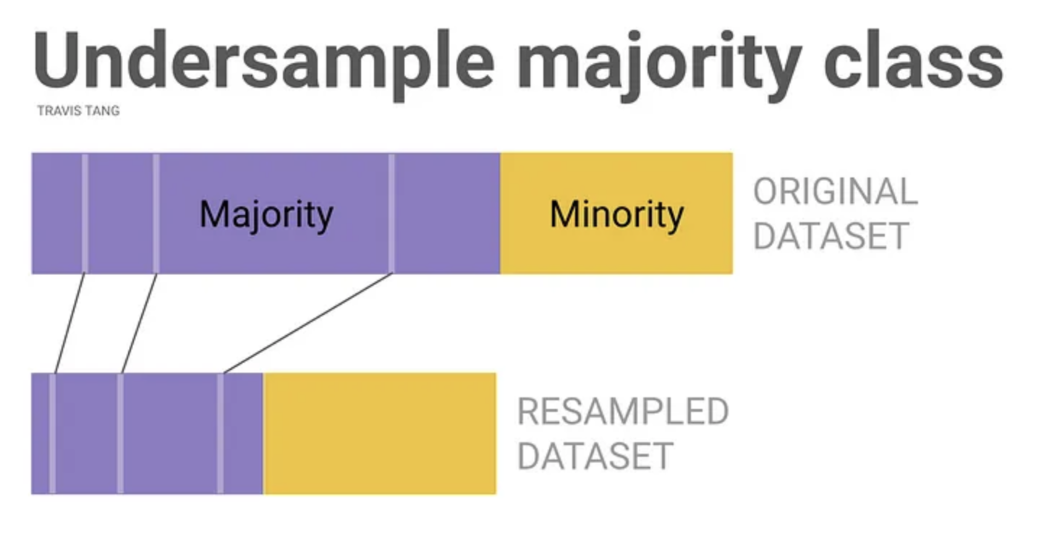
\includegraphics[width=0.8\linewidth]{Figure/Week 7/Down-sampling.png}
    \caption{Down-sampling}
\end{figure}

\noindent\textbf{Down-sampling}

Advantage: it does not introduce duplicates and/or artificial instances.

Disadvantages:

\begin{itemize}
    \item Not all data points are used.
    \item Potentially removing useful information.
\end{itemize}

Better choice for data with very high class imbalance.

\bigskip

\begin{figure}[h]
    \centering
    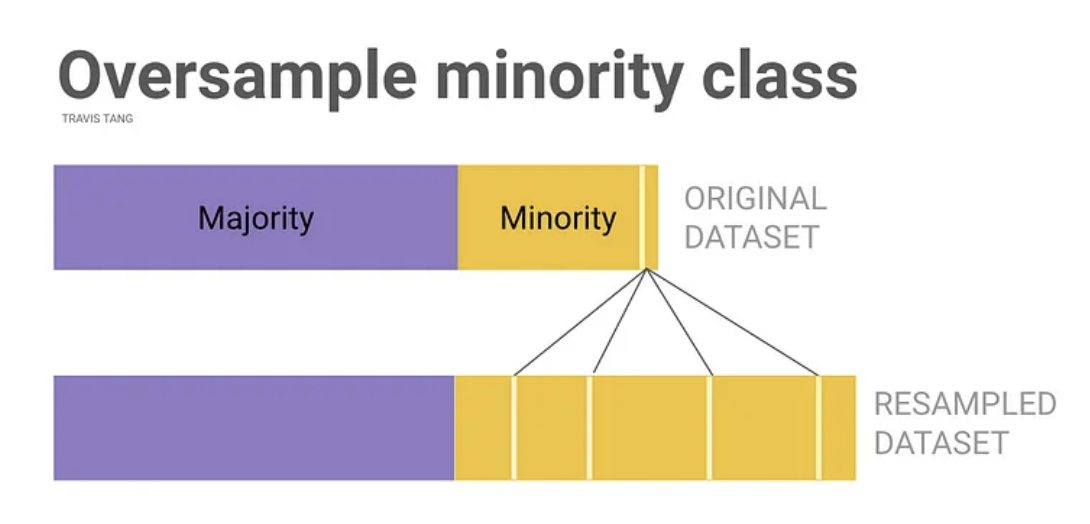
\includegraphics[width=0.8\linewidth]{Figure/Week 7/Up-sampling.png}
    \caption{Up-sampling}
\end{figure}

\noindent\textbf{Up-sampling}

Random up-sampling

Disadvantages:

\begin{itemize}
    \item creates duplicated and/or artificial instances
    \item can introduce bias and/or noise to the original data
\end{itemize}

\subsubsection{Create synthetic samples of the minority class}

\indent 

\textbf{Synthetic Minority Over-sampling Technique (SMOTE)} is a popular algorithm.

It creates synthetic samples from the minority class by:

\step Finding the $k$-nearest-neighbours for minority class observations.

\step Randomly choosing one of the $k$-nearest-neighbours, then using it to create a similar but random new observation.

Be careful that you split your data into training/test sets before doing any oversample/SMOTE. Otherwise, you will leak information from training to test data set.